\documentclass{article}
\usepackage[utf8]{inputenc}
\usepackage[top=2cm,bottom=2cm,left=2.2cm,right=2.2cm]{geometry}

\title{
{\Huge\bf COVID Assistant\\}
{\LARGE By Pandemic Hunters}
}
\author{\small Sinan Bingul, Anh H. Ngo, Fredy Zhang, Khoi T. Nguyen, Nam T. Hoang}
\date{April 11th, 2020}

\usepackage{natbib}
\usepackage{graphicx}

\begin{document}

\maketitle

\section*{Introduction}
Elderly people (65+) are one of the most vulnerable members of our community. They face many challenges during the COVID-19 pandemic. These challenges are;

\begin{itemize}
    \item Strict isolation policies.
    \item Obtaining essential resources .
    \item Obtaining relevant information or seeking help.
\end{itemize}


Elderly people may also have difficulties navigating through modern technology such as smartphones or computers. Hence we have developed a voice assistant that will help the elderly that requires minimal interaction with technology.


\section*{Solution}
The COVID Assistant is not envisioned to be a separate voice assistant to current options in the market such as Google Assistant or Amazon Alexa. Rather it is aimed to be an improvement/addition to these assistants.\\
 
The COVID Assistant will improve assistants in 4 different ways:
\begin{enumerate}
    \item Providing health suggestions by taking sensory inputs such as body temperature, heartbeat and cough sounds/patterns.
    \item Provides prediction and reporting about markets and parks human activity.
    \item Incorporating local shops with voice assistant.
    \item Including different parameters for predictions relevant to COVID-19 such as domestic and international travel information.
\end{enumerate}


The COVID Assistant will allow the elderly to obtain relevant health information in accordance with their cough patters and sounds, body temperature and heartbeat. It will help them avoid crowded locations and help them stay connected to their local shops.

\newpage

\section*{Possible technical implementation}
The voice assistant may collect body temperatures in many different ways. 

\begin{enumerate}
    \item It may measure body temperature through an inferred camera.
    \item It may integrate with a third-party hardware.
    \item It may have an onboard touch-sensitive hardware.
    \item It may simply take the user’s voice input.
\end{enumerate}

The voice assistant may recognise cough through machine learning and measure heartbeat through a red light sensor. Additional improvements may be in measuring respiratory vibration frequency as well through machine learning.\\

The underlying technology for reporting and predicting human activity exists in many different forms. Google is the market leader in providing this type of information through Google Maps for restaurants and roads. A collaboration with Google on extraction this data may allow this functionality to be implemented.\\

\begin{figure}
        \centering
        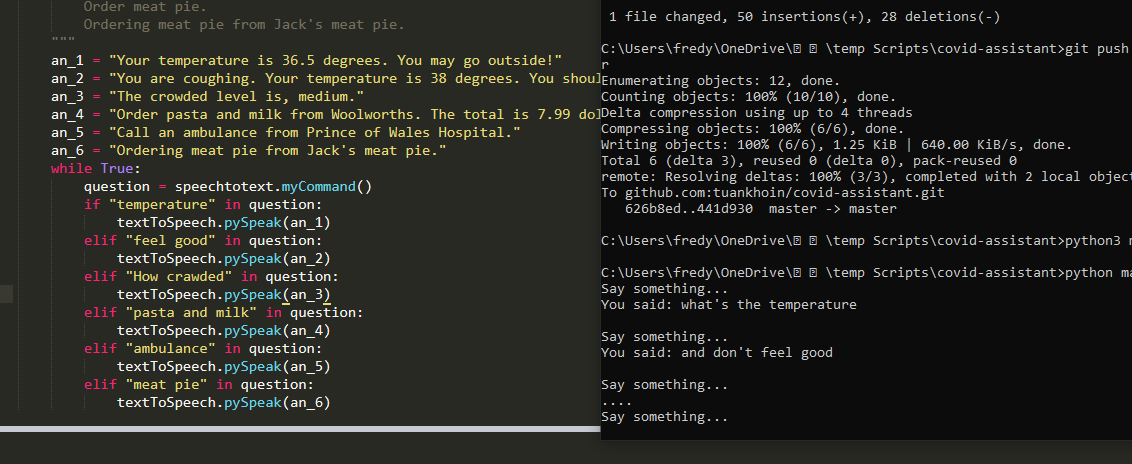
\includegraphics[scale=0.3]{code.png}
        \caption{A part of the speech implementation}
        \label{fig:GD}
\end{figure}

Incorporating local shops to voice assistants requires multiple steps and collaborations. The relevant IT infrastructure must be provided to the local shops. The delivery of the goods may be done via their own delivery service or a through a third party delivery service such as Uber Eats.

\begin{figure}
        \centering
        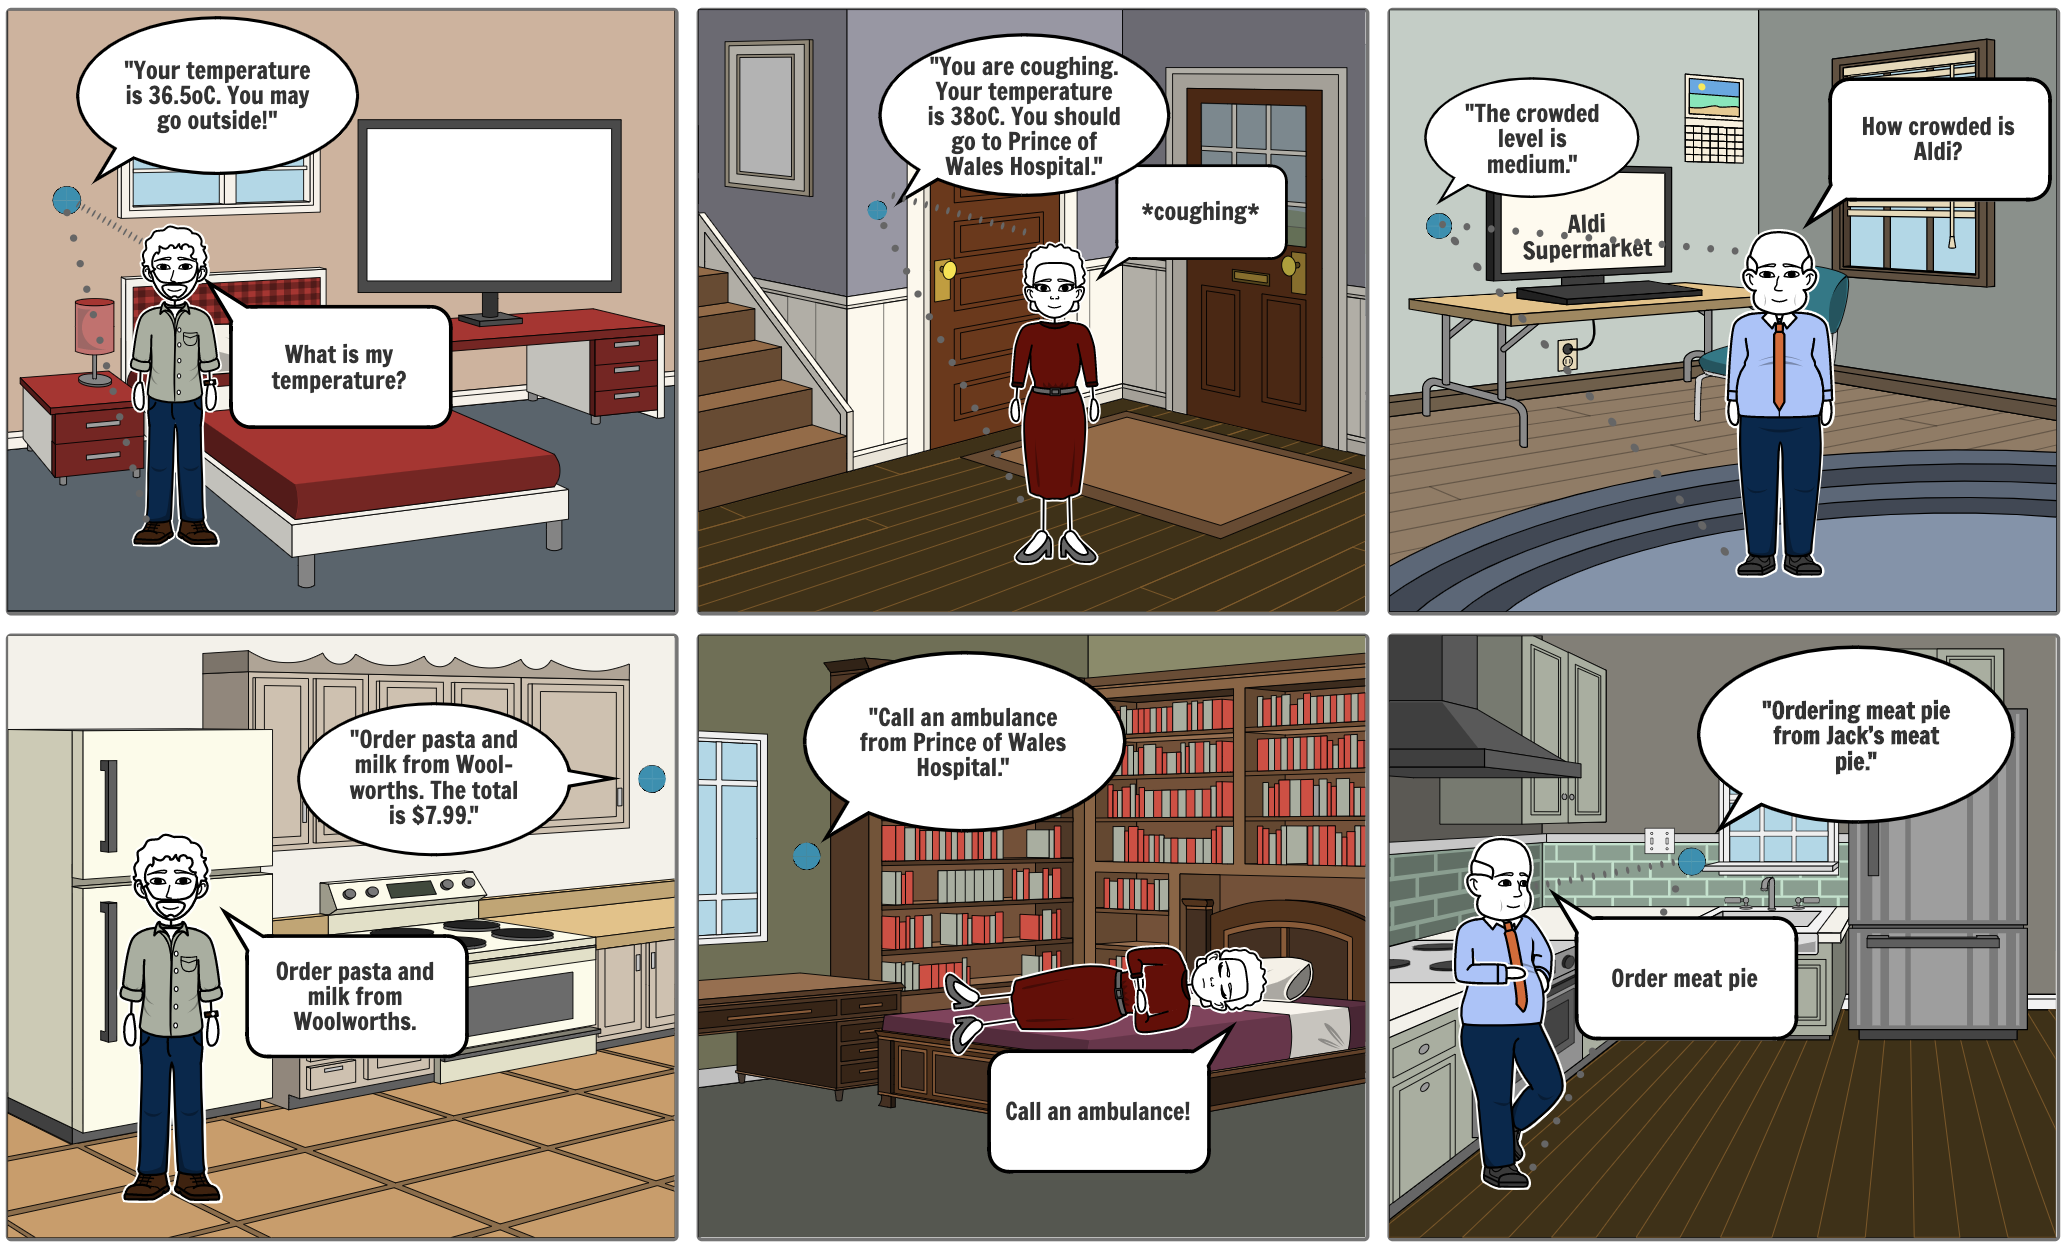
\includegraphics[scale=0.43]{scenario.png}
        \caption{Sample scenarios}
        \label{fig:GD}
\end{figure}

\newpage

\section*{Feasibility and limitations}

The implementation makes the assumption that an elderly person owns or will own a voice assistant. We believe our implementation will encourage the elderly to purchase a voice assistant, will encourage the loved ones to purchase it for them or the government providing it to the elderly. The low cost of assistants, large availability and the low learning curve will encourage the wide adoption of the device.

\end{document}
